\documentclass[10pt]{article}
\usepackage[cp1251]{inputenc}
\usepackage[english]{babel}
\usepackage[T2A]{fontenc}
\usepackage{graphicx}
\usepackage[mag=1000,a4paper,left=2.2cm,right=3.0cm,top=3.0cm,bottom=3.0cm]{geometry} % ,noheadfoot
\usepackage{enumerate}
\usepackage{pdflscape}
\usepackage{latexsym, amsgen, amsmath, amstext, amsbsy, amsopn, amsfonts, amsthm, amssymb, amscd}
\usepackage{mathtext}
\usepackage{mathrsfs}
\usepackage{wrapfig}



\title{COP-E Cognitive Architecture}
\author{Molchanov A.\,E., Markeeva L.\,B., Usvyatsov M.\,R.}
\usepackage[cp1251]{inputenc}
\usepackage[normalem]{ulem}
\usepackage{indentfirst}
\usepackage{grffile}
\usepackage{epstopdf}
\usepackage{makeidx}
\usepackage{verbatim}
\usepackage{tikz}
\usepackage{ulem}
\usetikzlibrary{arrows}
\usetikzlibrary{shapes}
\usetikzlibrary{positioning}
\usetikzlibrary{calc}
\usepackage{caption}
%\usepackage{graphicx,color}
\usepackage[T2A]{fontenc}
\usepackage{hyperref}
\graphicspath{{images/}}

\frenchspacing
\parindent=0.6cm
\parskip=2pt
\mathsurround=1pt

\sloppy
\newtheorem{df}{Definition}
\newtheorem{stmt}{Statement}

\newtheorem{notice}{Notice}
\newtheorem{theo}{Theorem}

\def\proof{{\indent Proof.}}


\newcommand{\itemi}[1]{\item \emph{#1} }

\begin{document}
\maketitle

\section{The COP-E Architecture}

The COP-E cognitive architecture is proposed for a cognitive humanoid law-enforcement robot. 

A robot that implements the architecture should be capable of turning (\emph{developing}) into a highly-efficient detective able to think about crimes (drawing conclusions that would lead to uncovering a culprit), act to reveal information, and actively prevent crimes. A robot would be working in real world, with no limitations to the environment. It would benefit from external communication like radio frequency communications, but these links are optional.

Since the architecture is emergent, enactive and embodied, much attention is put into action-perception interconnection and motivated development.

The emergent approach was chosen as the most perspective in the area of cognitive systems, plus in the application domain of the robot as much cognition as possible is required. Only emergent systems allow for explicit system development. This justifies the inapplicability of the cognitivists� approach. The system could possibly be hybrid, and can to some extent be considered hybrid for the presence of some almost symbolic knowledge. However, the usage of such knowledge is extremely restricted in the system. In fact, the system evolves to understand the predefined ``almost symbolic�� knowledge and converts it freely into non-symbolic knowledge.

The architecture describes basic modules that comprise a robot, including ``brain'' and ``body'' parts. 

There is no explicit distinction between brain and body, however some modules (such as the goal module) can be attributed to brain, some (sensors) can be attributed to body. Modules are tightly interconnected using various links with no predefined data format. There are just some limitations on data being passed, plus there is an error component that is included in almost all data.

The modular structure of the architecture is presented on the picture \ref{fig:modules}. Brain and body parts are separated, however the separation is vague.
\begin{landscape}
\begin{figure}[h!]
	\center{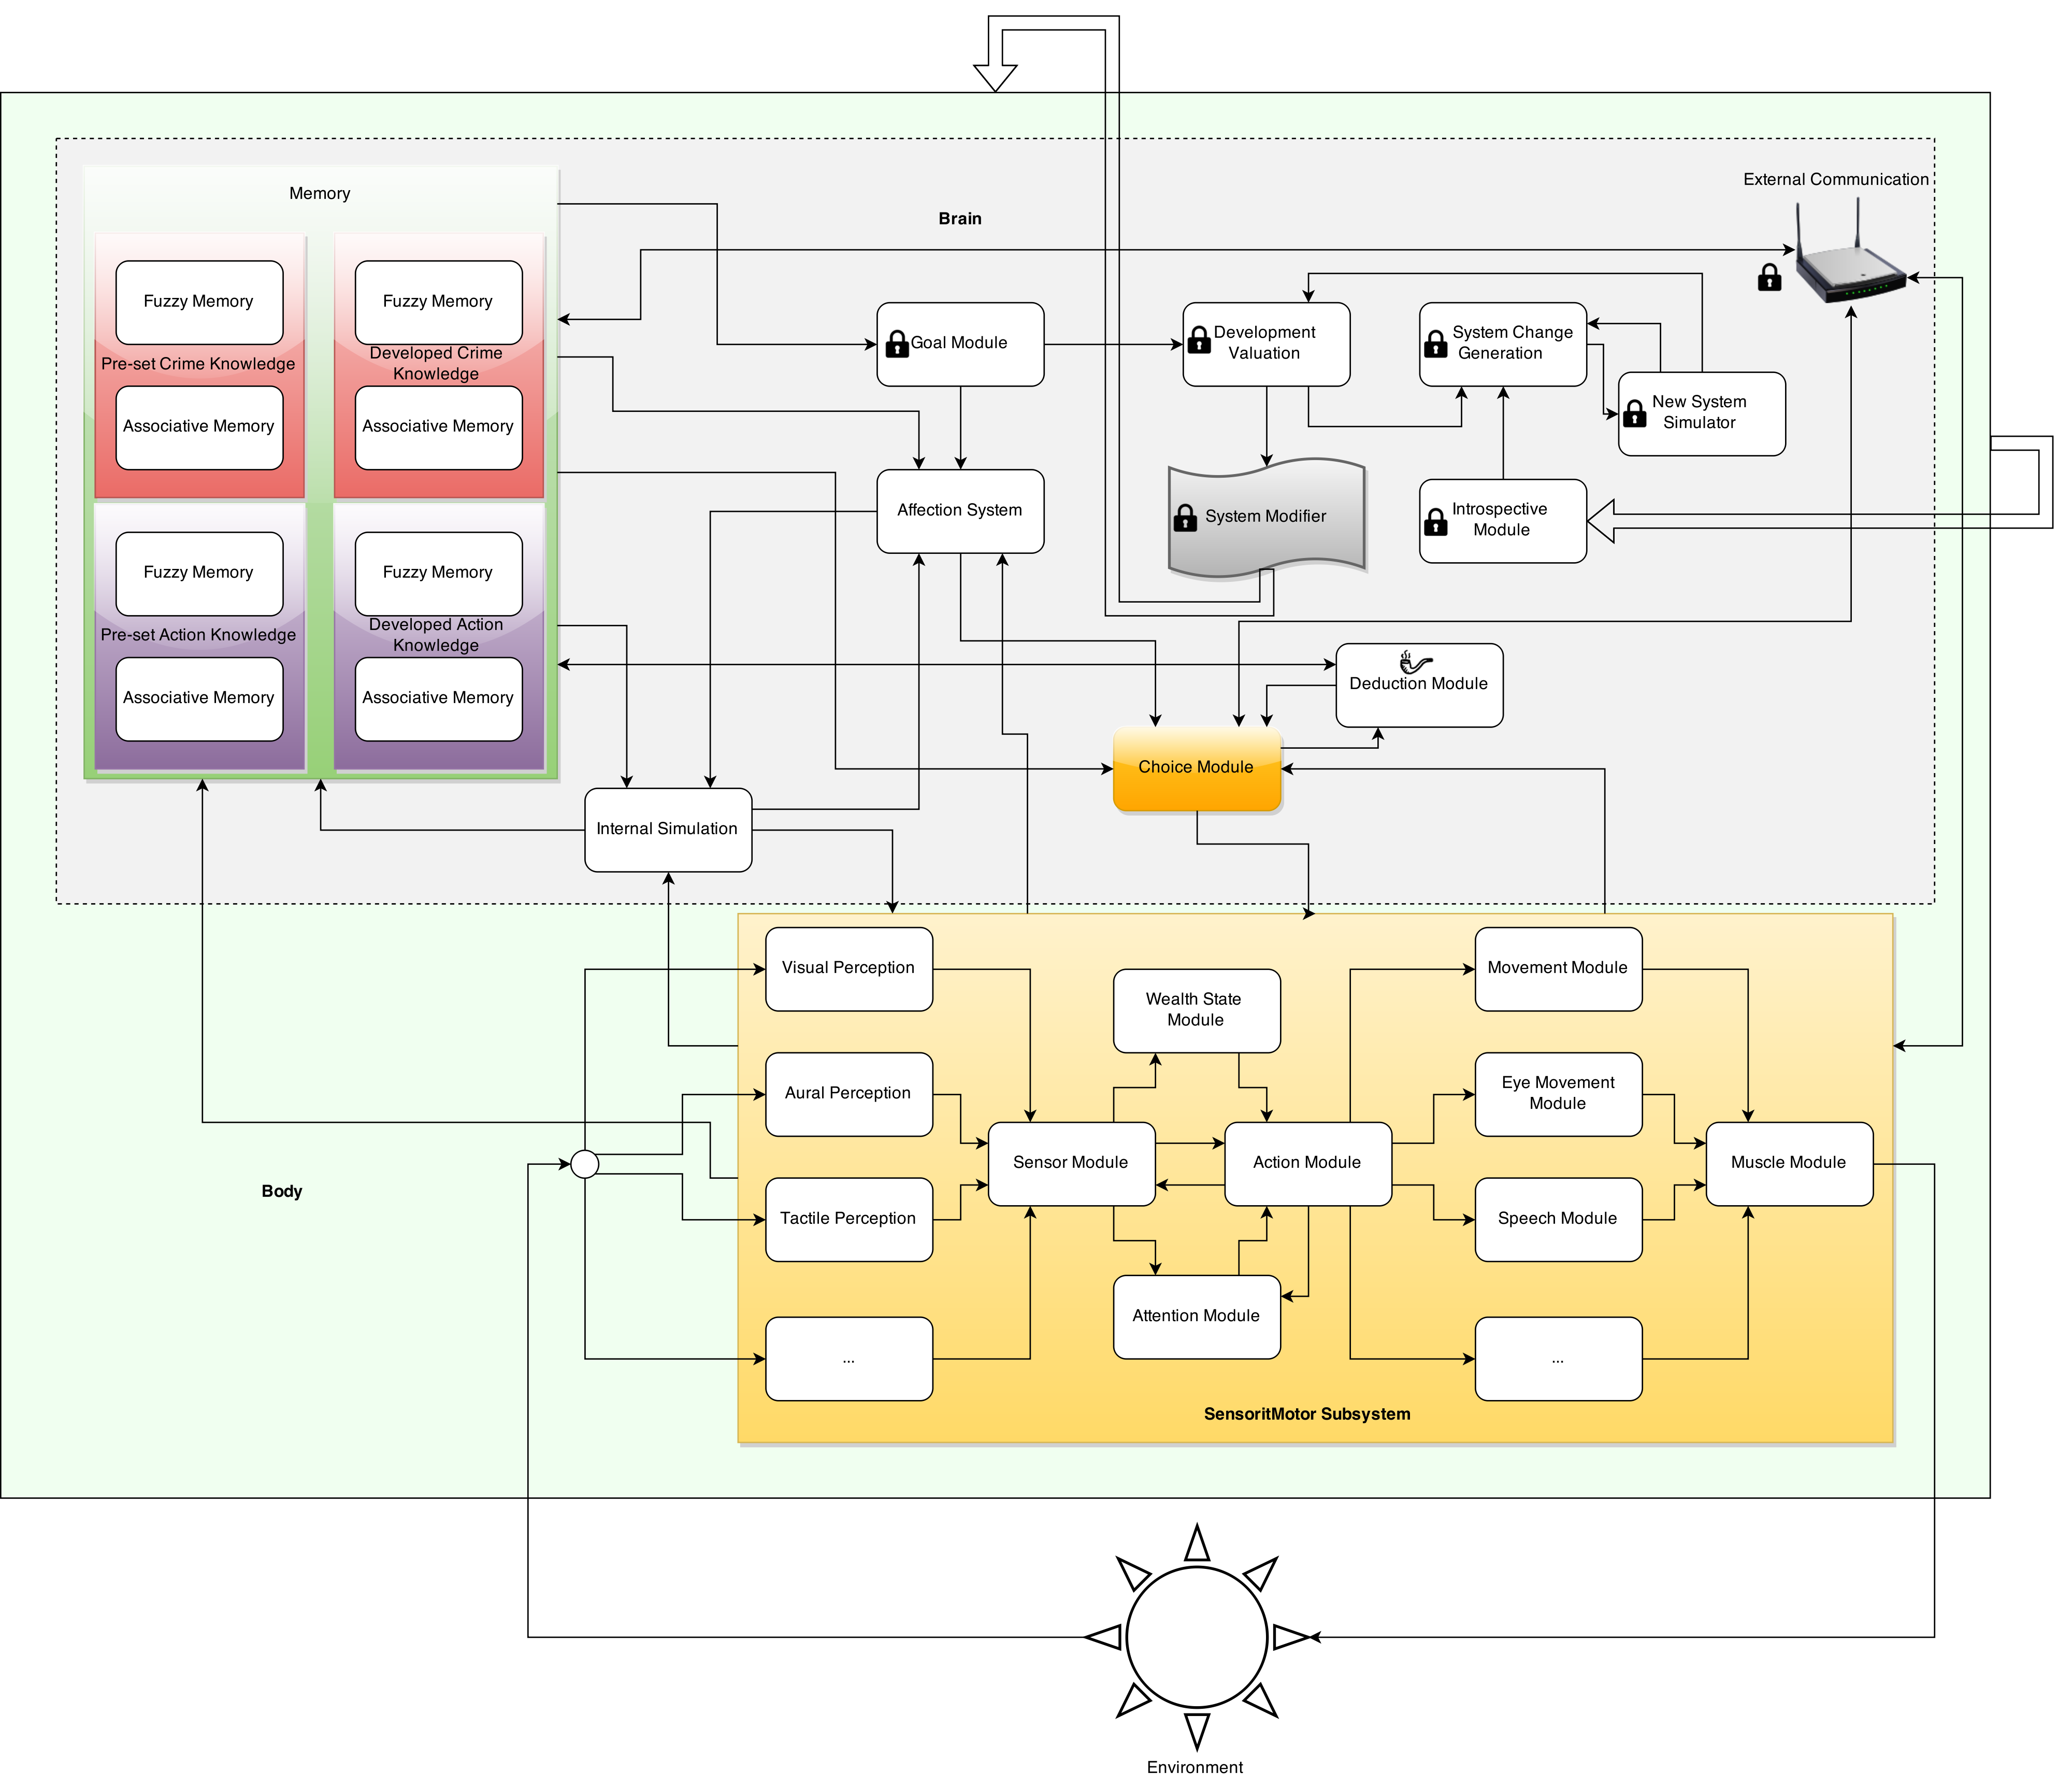
\includegraphics[width=0.7\paperheight]{arch}}
	\caption{COP-E structure}
	\label{fig:modules}
\end{figure}
\end{landscape}

Following is a brief description of the system constitution.

\subsection{Decision Making}

The most important question a cognitive system must answer is \emph{what to do now?} The module responsible for this answer is the choice module. This module has inputs from systems which affect what decision to make. Memory provides information about possible actions that can be performed. The actions are evaluated basing on the affection module, which is in turn influenced by the goal module. No direct goal-choice connection is made because the architecture does its best to eradicate any form of predefined knowledge. Goals of a law-enforcing robot must be stated explicitly and externally, so there needs to be a mechanism for knowledge negotiation between a robot and its constructor. This is implemented in a goal-memory interconnection, with memory containing some predefined knowledge. 

The choice module is not connected with an internal simulation module, because the latter is used in separation and works through memory. 

There is, however, a connection from the sensorimotor subsystem. This is due to the fact that the system is embodied and the current state of the sensorimotor subsystem, including all its subcomponents, interferes with the decision making both in the valuation of possible action and in the set of possible actions itself. 

Once the system has a set of possible actions to do, a valuation of these actions and the action subsystem to carry out these actions, the system is the desired robot. The question now is how to implement these components and the ability to change (develop and learn).

\subsection{Memory}

The memory subsystem contains two basic memory types -- associative and fuzzy. 

Associative memory gets any input and provides data that is in some sense similar. The way how it does so is undefined for it is a subject to change. Initially techniques from machine learning such as clustering and neural networks are applied. Once the system develops new techniques for associative memory, the initial techniques can be disabled (by the choice of the system).

Fuzzy memory introduces some randomness to memory. It is able to randomly generate data not directly related to the input. However, input is taken into account at least for information valuation. Not all information is stored in memory forever. Each element has a degree of importance (which effectively makes the memory fuzzy) and once the degree drops below a threshold it is discarded. The degrees affect the frequency of this data retrieval. So, elements with bigger degree are output more frequently. Every element can be referenced in an associative manner, increasing its degree. All degrees drop in time, so the less frequently the element is accessed associatively, the less degree it gets. The memory performs internal data processing basing on fuzzy logic for drawing new data, but the process is mostly random.

The combination of memories allows to fetch relevant information efficiently still allowing for some randomness.

There is another division in memory. The system has inbuilt memory of its actions (which is gathered with a controlled simulation) and of historical crimes and their solutions. The former allows the system to make some initial actions and is very limited for controlled evolution is hard to convey. The historical crimes information is on the other hand quite rich but in some term senseless for the system unless it develops an understanding of it. Once the understanding is developed, the system can use the information for action generation, valuation, and for anticipation. 

Another part of memory is the developed memory. This contains all information the system has gathered and is undefined in terms of the architecture as it belongs to the developmental phase. However, initially the system is advised to divide memory into action and ``crime logic'' sections, i.e. the action subsystem has stronger linkage to action memory and the choice module is stronger linked to the crime memory.

\subsection{Affection}

The system is mostly driven by affection. This module is relatively complex as it is able to compare the current state to the goal state, infer possible actions' outcome basing on memory from internal simulation module and evaluate the current body state (i.e. wealth). This includes an endocrine-like system which additionally maintains homeostasis via favouring actions that maintain the system state rather than disrupt it. 

No additional homeostatic module is introduced as it could possibly overcome the goal module and make the robot too autonomous.

\subsection{Sensorimotor Subsystem}

Since the cognitive architecture is embodied, the system includes an explicit body with its perception and action interconnected systems. The sensorimotor system as a whole is connected to the memory (for action/perception information is stored in the memory), to the internal simulation module for it should be able to predict outcomes of actions accurately in terms of bodily events, to the affection module for current state information, and to the choice module for proper decision making.

The subsystem contains separated perception modules for various input systems, including but not limited to, visual, aural, and tactile perception modules. The system likewise contains separate action modules like movement and speech. All perception and action modules are connected to dedicated and interconnected perception and action modules with separate wealth state module and attention module.

\subsection{Development}

The architecture explicitly states the ability to develop. It has a set of modules that are used for new system layouts generation, valuation and application. Given information of the current state (via introspective module), the system chooses a new configuration which includes a rearrangement of modules and/or module creation and/or module removal. These new systems are modelled with a separate module and valuated with help of the goal module. Once a development decision modules thinks it is appropriate for the system to be changed, the change is applied. Modules marked with a lock on the diagram are never changed in development for that would threaten the goal-making. In fact, the system can potentially develop a completely disconnected system that would work on its own, and that�s where the goal module comes into play. Any modification that cuts off the goal module from the action module is prohibited. The test is performed with a Petri nets analysis in the development valuation module with assistance of the goal module.

\subsection{Autonomy}

The cognitive architecture is developed to be autonomous to some extent. It maintains basic homeostasis, plus it takes care of resource acquiring on its own. It does its best to overcome any precarious environment conditions, unless it violates its goal of law-enforcement. So, generally, the goal module is not autonomous in the sense that it is pre-defined by the creator. 

There is another breach in the autonomy, it is the external communication. This module allows a human operator to overcome any robot�s system, including its goal subsystem and to carry on any action the operator wants, including memory modification, choice enforcement or a low-level action. This is non-negotiable with a robot, so it is troublesome to implement on the high-level, thus the intervention is mostly low-level. 

The external communication is also used for the robot high-level communication with humans. So, in fact, it is partly another action-perception submodule.

Additionally, this module sends information about all information from robot�s low-level sensors for humans to be aware of robot�s location, state and actions. 

If the external robot control is an emergency system for a robot, the communication and sensors information feeding are normal working processes.
\pagebreak
\subsection{Nature of Knowledge}

The knowledge each component temporarily stores is non-symbolic non-grounded information. All information is retrieved and stored associatively and fuzzily. No explicit world representation is created, however a knowledge about the world emerges on its own while the robot explores the world. This process is not controlled but is modulated by the goal and affection modules. 

Memory stores information as a flow of data with connections between pieces. No specific ``chunk�� is defined. However, data is vaguely typed as mentioned above.

\subsection{Nature of Connections}

Connections are all weighted with adjustable weights. Each connection is not a single stream of data but a set of channels each of which can send data (sometimes in duplex mode). All data is represented as a flow of information encoded in some way (though the encoding is not explicitly defined). Some information is chemical in terms of the endocrine system, some information is electric impulses. 
No specific input-output for modules is defined as it is a subject to change. However, initial configuration is specified and is presented on the diagram with thin lines representing specific information and wide lines representing information or modification of the system as a whole.

\subsection{Deduction Module}
\begin{wrapfigure}{l}{0.08\textwidth}

\includegraphics[width=0.08\textwidth]{pipe}
\end{wrapfigure}
This module is a tribute to Sherlock Holmes, the famous detective. The module smokes internally and tries to explain everything with a deduction (which is, in fact, \emph{induction}). The module does not affect the robot in any way since all reasoning is performed in other modules as described earlier. 

\section {Characteristics}

The COP-E architecture can be characterized according to the following table.

\begin{tabular}{|c|c|p{300pt}|}
	\hline
	Property & Value & Reason \\
	\hline
	Embodiment & x & Explicit embodiment\\
	\hline
	Perception & x & Explicit perception and action-perception interconnectedness\\
	\hline
	Action & x & Explicit action and action-perception interconnectedness\\
	\hline
	Anticipation & + & Internal simulation for anticipation connected to memory and the sensorimotor subsystem, however no explicit mechanics for internal simulation are given \\
	\hline
	Adaptation & x & Detailed description of development and learning\\ 
	\hline
	Motivation & x & The goal module specifies motivation alongside with the affection module\\
	\hline
	Autonomy & x & Autonomy is required for the system, but is necessarily limited for goal-perseverance \\
	\hline
	
\end{tabular}
\pagebreak
\begin{figure}[h!]
	\center{
\includegraphics[width=1\textwidth]{space}}
	\caption{COP-E Abstraction-Inspiration Space}
	\label{fig:space}
\end{figure}

The location of the COP-E architecture in the Abstraction-Inspiration space is presented on the figure \ref{fig:space}. 


The architecture is inspired by both biological cognition (in the system interconnectedness, associative memory, endocrine system, homeostasis, and affection). However some parts are borrowed from the computational domain, such as the fuzzy sets, Petri nets for system evaluation, and data analysis for associative memory \emph{initial} implementation.

The abstraction level is moderately high as no direct computation mechanisms are provided, plus data flows are of high level. No detailed affection system is provided either. 

\section{Student Participation}

The assignment is completed by a group of three students, Andrei Molchanov, Larisa Markeeva and Mikhail Usvyatsov. The per-student description of solved tasks is as follows.

\begin{itemize}
	\item Mikhail Usvyatsov: The paradigm choice, the application domain specification, the high-level design of the system, help in diagram creation, the data flow design.
	\item Larisa Markeeva: The memory subsystem, the sensorimotor and decision making subsystems development, the overall analysis.
	\item Andrei Molchanov: The developmental subsystem, interconnectedness development with aid from Mikhail, final text and diagrams preparation. The deduction module.
\end{itemize}

\end{document}